% Options for packages loaded elsewhere
\PassOptionsToPackage{unicode}{hyperref}
\PassOptionsToPackage{hyphens}{url}
%
\documentclass[
]{article}
\usepackage{amsmath,amssymb}
\usepackage{lmodern}
\usepackage{ifxetex,ifluatex}
\ifnum 0\ifxetex 1\fi\ifluatex 1\fi=0 % if pdftex
  \usepackage[T1]{fontenc}
  \usepackage[utf8]{inputenc}
  \usepackage{textcomp} % provide euro and other symbols
\else % if luatex or xetex
  \usepackage{unicode-math}
  \defaultfontfeatures{Scale=MatchLowercase}
  \defaultfontfeatures[\rmfamily]{Ligatures=TeX,Scale=1}
\fi
% Use upquote if available, for straight quotes in verbatim environments
\IfFileExists{upquote.sty}{\usepackage{upquote}}{}
\IfFileExists{microtype.sty}{% use microtype if available
  \usepackage[]{microtype}
  \UseMicrotypeSet[protrusion]{basicmath} % disable protrusion for tt fonts
}{}
\makeatletter
\@ifundefined{KOMAClassName}{% if non-KOMA class
  \IfFileExists{parskip.sty}{%
    \usepackage{parskip}
  }{% else
    \setlength{\parindent}{0pt}
    \setlength{\parskip}{6pt plus 2pt minus 1pt}}
}{% if KOMA class
  \KOMAoptions{parskip=half}}
\makeatother
\usepackage{xcolor}
\IfFileExists{xurl.sty}{\usepackage{xurl}}{} % add URL line breaks if available
\IfFileExists{bookmark.sty}{\usepackage{bookmark}}{\usepackage{hyperref}}
\hypersetup{
  pdftitle={Korea Income Distribution 2010},
  pdfauthor={coop711},
  hidelinks,
  pdfcreator={LaTeX via pandoc}}
\urlstyle{same} % disable monospaced font for URLs
\usepackage[margin=1in]{geometry}
\usepackage{graphicx}
\makeatletter
\def\maxwidth{\ifdim\Gin@nat@width>\linewidth\linewidth\else\Gin@nat@width\fi}
\def\maxheight{\ifdim\Gin@nat@height>\textheight\textheight\else\Gin@nat@height\fi}
\makeatother
% Scale images if necessary, so that they will not overflow the page
% margins by default, and it is still possible to overwrite the defaults
% using explicit options in \includegraphics[width, height, ...]{}
\setkeys{Gin}{width=\maxwidth,height=\maxheight,keepaspectratio}
% Set default figure placement to htbp
\makeatletter
\def\fps@figure{htbp}
\makeatother
\setlength{\emergencystretch}{3em} % prevent overfull lines
\providecommand{\tightlist}{%
  \setlength{\itemsep}{0pt}\setlength{\parskip}{0pt}}
\setcounter{secnumdepth}{-\maxdimen} % remove section numbering
\ifluatex
  \usepackage{selnolig}  % disable illegal ligatures
\fi

\title{Korea Income Distribution 2010}
\author{coop711}
\date{2021-03-28}

\begin{document}
\maketitle

\hypertarget{data}{%
\subsection{Data}\label{data}}

자료 입력

\begin{verbatim}
(income_kr <- read.table("../data/labor_income_kor.txt", 
                         header = TRUE, 
#                          encoding = "UTF-8",
                         row.names = 1))
\end{verbatim}

\begin{verbatim}
##          Earners... Income...
## 0-5            19.1       1.7
## 5-10           12.3       3.6
## 10-20          22.8      12.8
## 20-30          14.4      13.6
## 30-40           9.8      13.0
## 40-60          12.0      22.5
## 60-80           5.4      14.1
## 80-100          2.3       7.8
## 100-200         1.6       7.7
## 200-300         0.1       1.2
## 300-500         0.1       0.8
## 500-1000        0.0       0.6
## 1000-           0.0       0.6
\end{verbatim}

\begin{verbatim}
str(income_kr)
\end{verbatim}

\begin{verbatim}
## 'data.frame':    13 obs. of  2 variables:
##  $ Earners...: num  19.1 12.3 22.8 14.4 9.8 12 5.4 2.3 1.6 0.1 ...
##  $ Income... : num  1.7 3.6 12.8 13.6 13 22.5 14.1 7.8 7.7 1.2 ...
\end{verbatim}

변수명을 조정하고, 다시 확인.

\begin{verbatim}
names(income_kr) <- c("Earners(%)", "Income(%)")
income_kr
\end{verbatim}

\begin{verbatim}
##          Earners(%) Income(%)
## 0-5            19.1       1.7
## 5-10           12.3       3.6
## 10-20          22.8      12.8
## 20-30          14.4      13.6
## 30-40           9.8      13.0
## 40-60          12.0      22.5
## 60-80           5.4      14.1
## 80-100          2.3       7.8
## 100-200         1.6       7.7
## 200-300         0.1       1.2
## 300-500         0.1       0.8
## 500-1000        0.0       0.6
## 1000-           0.0       0.6
\end{verbatim}

\begin{verbatim}
rownames(income_kr) <- sub(pattern = "-", 
                           replacement = " - ", 
                           x = rownames(income_kr))
# kable(income_kr)
\end{verbatim}

\texttt{barplot()} 을 그리기 위하여 \texttt{height}를 설정하려면
\texttt{width}를 파악하여야 함. 그러기 위해서 소득 구간을
\texttt{rownames}의 구간으로부터 설정. \texttt{strsplit()}의 활용방법
확인,

\begin{verbatim}
(r_names_split <- strsplit(rownames(income_kr), 
                           split = " - "))
\end{verbatim}

\texttt{{[}{]}}, \texttt{{[}{[}{]}{]}}의 차이와 \texttt{{[}{]}}를 함수로
표현하는 방법에
유의(\texttt{results\ =\ \textquotesingle{}hide\textquotesingle{}}를
지우고 실행).

\begin{verbatim}
r_names_split[1]
r_names_split[1][[1]]
r_names_split[[1]]
r_names_split[[1]][1]
`[`(r_names_split, 1)
`[[`(r_names_split, 1)
\end{verbatim}

\texttt{anonymous\ function}과 \texttt{sapply()}를 이용하여 긴 character
list의 앞 원소만 추출하는 방법을 살필 것.

\begin{verbatim}
# (r_names_split_first <- sapply(r_names_split, function(x){x[1]}))
(r_names_split_first <- sapply(r_names_split, 
                               FUN = `[`, 1))
\end{verbatim}

\begin{verbatim}
##  [1] "0"    "5"    "10"   "20"   "30"   "40"   "60"   "80"   "100"  "200" 
## [11] "300"  "500"  "1000"
\end{verbatim}

\begin{verbatim}
(income_breaks <- as.numeric(r_names_split_first))
\end{verbatim}

\begin{verbatim}
##  [1]    0    5   10   20   30   40   60   80  100  200  300  500 1000
\end{verbatim}

\begin{verbatim}
(income_breaks <- c(income_breaks, 2000))
\end{verbatim}

\begin{verbatim}
##  [1]    0    5   10   20   30   40   60   80  100  200  300  500 1000 2000
\end{verbatim}

\texttt{width}에 해당하는 각 소득구간의 폭을 계산

\begin{verbatim}
(income_widths <- diff(income_breaks))
\end{verbatim}

\begin{verbatim}
##  [1]    5    5   10   10   10   20   20   20  100  100  200  500 1000
\end{verbatim}

각 기둥의 면적이 해당 소득구간의 퍼센티지와 같게 해주려면 각 퍼센티지를
\texttt{width}로 나눠줘야 함. 다음 각 경우를
비교(\texttt{results\ =\ \textquotesingle{}hide\textquotesingle{}}를
지우고 실행).

\begin{verbatim}
options(digits = 3)
(height_earners <- income_kr[, 1]/income_widths)
(height_earners_2 <- income_kr[, "Earners(%)"]/income_widths)
(height_earners_3 <- income_kr[[1]]/income_widths)
(height_earners_4 <- income_kr[1]/income_widths)
(height_earners_5 <- income_kr["Earners(%)"]/income_widths)
\end{verbatim}

\hypertarget{probability-historam-with-barplot}{%
\subsection{\texorpdfstring{Probability Historam with
\texttt{barplot()}}{Probability Historam with barplot()}}\label{probability-historam-with-barplot}}

아무런 \texttt{argument} 도 설정하지 않고 \texttt{barplot()} 을 그리면

\begin{verbatim}
barplot(height_earners, 
        width = income_widths)
\end{verbatim}

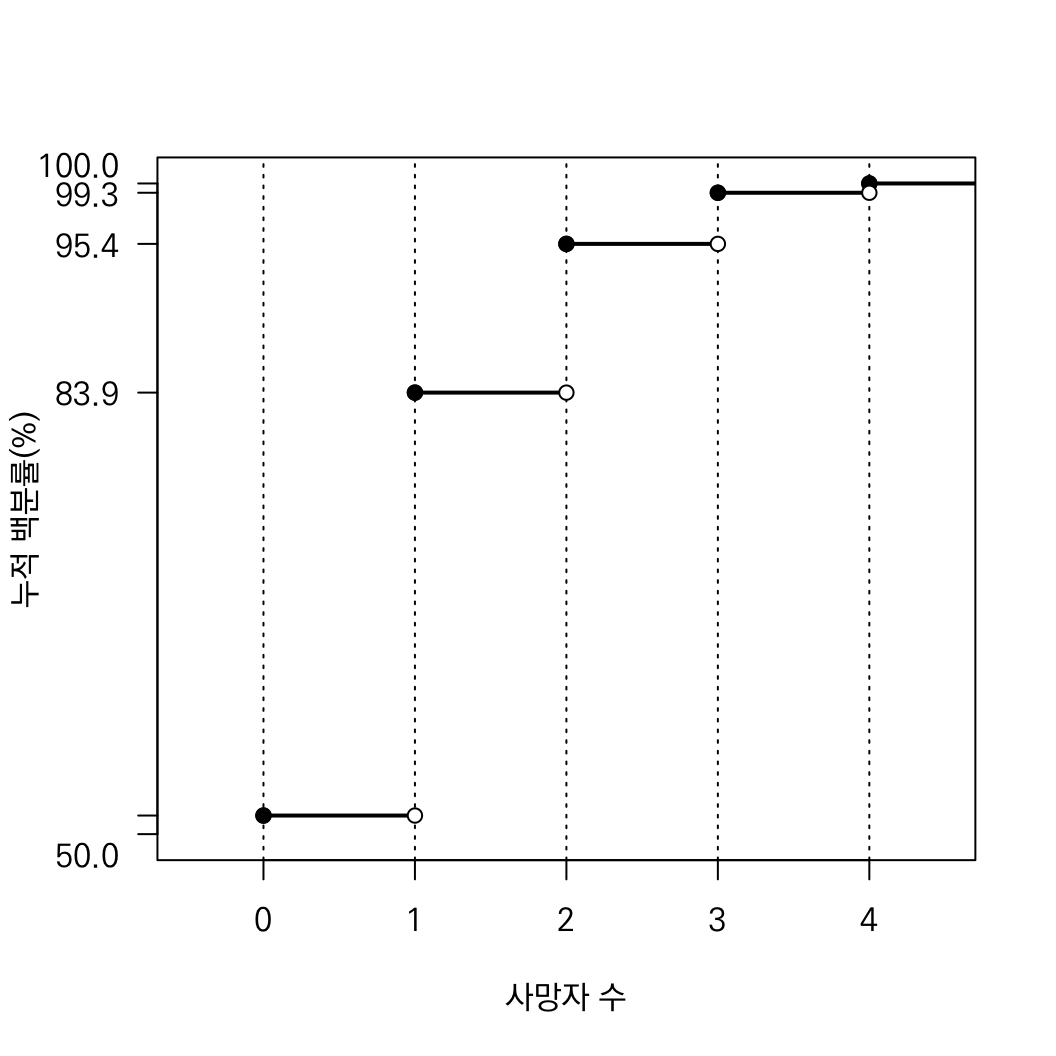
\includegraphics{Korea_Income_gini_2010_files/figure-latex/unnamed-chunk-5-1.pdf}

각 막대의 이름을 \texttt{rownames}에서 가져오면

\begin{verbatim}
(names_bar <- rownames(income_kr))
\end{verbatim}

\begin{verbatim}
##  [1] "0 - 5"      "5 - 10"     "10 - 20"    "20 - 30"    "30 - 40"   
##  [6] "40 - 60"    "60 - 80"    "80 - 100"   "100 - 200"  "200 - 300" 
## [11] "300 - 500"  "500 - 1000" "1000 - "
\end{verbatim}

막대의 이름을 넣어 다시 그리되, 막대 사이의 공간을 없애면

\begin{verbatim}
barplot(height_earners, 
        width = income_widths, 
        space = 0, 
        names.arg = names_bar)
\end{verbatim}

\includegraphics{Korea_Income_gini_2010_files/figure-latex/barplot no space-1.pdf}

실제 인원은 거의 없는 것처럼 보이는 5억원 이상의 구간을 합쳐야 할 필요.
자료를 재구성하면,

\begin{verbatim}
income_kr_2 <- income_kr[1:11, ]
income_kr_2[11, ] <- apply(income_kr[11:13, ], 
                           MARGIN = 2, 
                           FUN = sum)
income_kr_2
\end{verbatim}

\begin{verbatim}
##           Earners(%) Income(%)
## 0 - 5           19.1       1.7
## 5 - 10          12.3       3.6
## 10 - 20         22.8      12.8
## 20 - 30         14.4      13.6
## 30 - 40          9.8      13.0
## 40 - 60         12.0      22.5
## 60 - 80          5.4      14.1
## 80 - 100         2.3       7.8
## 100 - 200        1.6       7.7
## 200 - 300        0.1       1.2
## 300 - 500        0.1       2.0
\end{verbatim}

\begin{verbatim}
rownames(income_kr_2)
\end{verbatim}

\begin{verbatim}
##  [1] "0 - 5"     "5 - 10"    "10 - 20"   "20 - 30"   "30 - 40"   "40 - 60"  
##  [7] "60 - 80"   "80 - 100"  "100 - 200" "200 - 300" "300 - 500"
\end{verbatim}

\begin{verbatim}
rownames(income_kr_2)[11] <- "300 -  "
income_kr_2
\end{verbatim}

\begin{verbatim}
##           Earners(%) Income(%)
## 0 - 5           19.1       1.7
## 5 - 10          12.3       3.6
## 10 - 20         22.8      12.8
## 20 - 30         14.4      13.6
## 30 - 40          9.8      13.0
## 40 - 60         12.0      22.5
## 60 - 80          5.4      14.1
## 80 - 100         2.3       7.8
## 100 - 200        1.6       7.7
## 200 - 300        0.1       1.2
## 300 -            0.1       2.0
\end{verbatim}

\begin{verbatim}
(income_breaks_2 <- income_breaks[1:12])
\end{verbatim}

\begin{verbatim}
##  [1]   0   5  10  20  30  40  60  80 100 200 300 500
\end{verbatim}

\begin{verbatim}
income_widths_2 <- diff(income_breaks_2)
height_earners_2 <- income_kr_2[, 1]/income_widths_2
names_bar_2 <- rownames(income_kr_2)
\end{verbatim}

다시 \texttt{barplot()}을 작동시키되 회색 대신 흰색을 넣고, 막대 사이의
공간을 없애고 제목과 축이름을 붙이면

\begin{verbatim}
title_1 <- "Korea Income Wage Earners' Distribution"
xlab_1 <- "Income Class (Million Won)"
ylab_1 <- "% per Million Won"
barplot(height_earners_2, 
        width = income_widths_2, 
        names.arg = names_bar_2, 
        space = 0, 
        col = "white")
title(main = title_1, 
      xlab = xlab_1, 
      ylab = ylab_1)
\end{verbatim}

\includegraphics{Korea_Income_gini_2010_files/figure-latex/unnamed-chunk-7-1.pdf}

1억 이상의 구간을 합치기 위하여 자료를 다시 손보면,

\begin{verbatim}
income_kr_3 <- income_kr_2[1:9, ]
income_kr_3[9, ] <- apply(income_kr_2[9:11, ], 2, sum)
rownames(income_kr_3)[9] <- "100 -   "
income_breaks_3 <- income_breaks_2[-(11:12)]
income_widths_3 <- diff(income_breaks_3)
height_earners_3 <- income_kr_3[, 1]/income_widths_3
names_bar_3 <- rownames(income_kr_3)
\end{verbatim}

1억 이상의 구간을 합쳐 barplot을 그리면,

\begin{verbatim}
barplot(height_earners_3, 
        width = income_widths_3, 
        names.arg = names_bar_3, 
        space = 0, 
        col = "white")
title(main = title_1, 
      xlab = xlab_1, 
      ylab = ylab_1)
\end{verbatim}

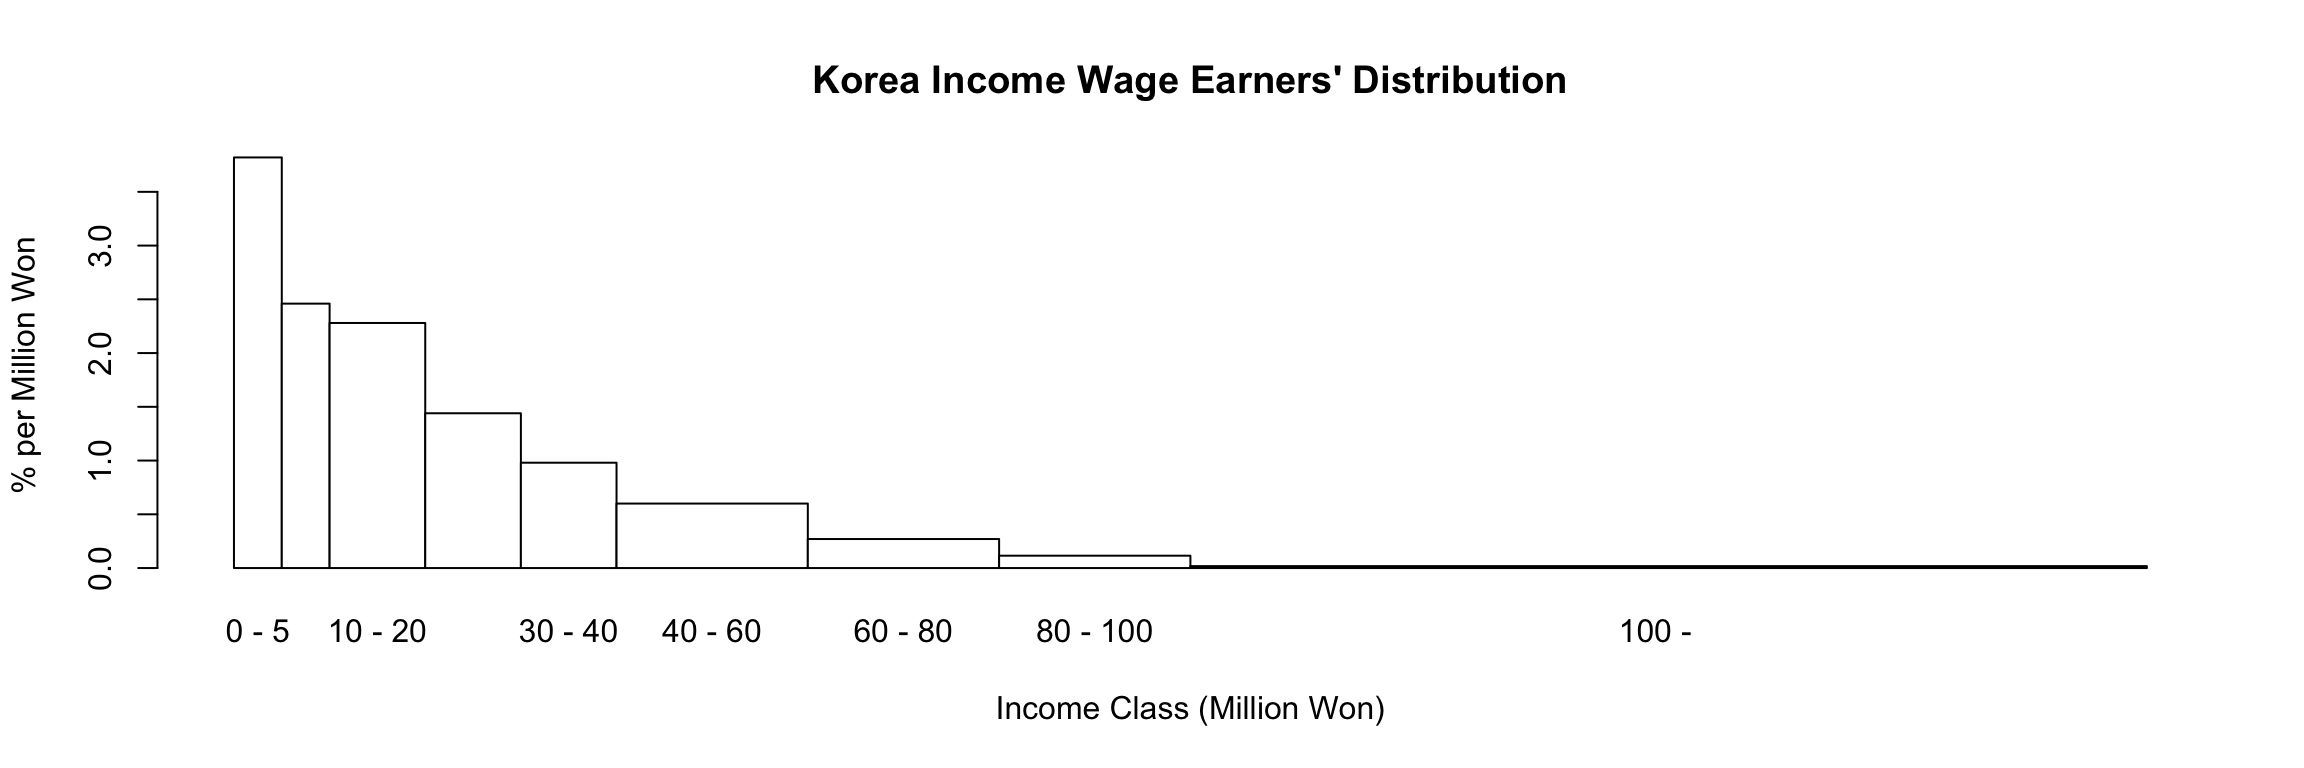
\includegraphics{Korea_Income_gini_2010_files/figure-latex/barplot 3-1.pdf}

같은 방법으로 소득규모에 대하여 세 개의 \texttt{barplot}을 그리려면,
우선 자료를 정리하고.

\begin{verbatim}
height_income <- income_kr[, 2]/income_widths
height_income_2 <- income_kr_2[, 2]/income_widths_2
height_income_3 <- income_kr_3[, 2]/income_widths_3
\end{verbatim}

세 개의 barplot을 한 화면에 연속적으로 그리기 위하여
\texttt{par(mfrow\ =\ c(3,\ 1))} 설정

\begin{verbatim}
par(mfrow = c(3, 1))
barplot(height_income, 
        width = income_widths, 
        names.arg = names_bar, 
        space = 0, 
        col = "white")
barplot(height_income_2, 
        width = income_widths_2, 
        names.arg = names_bar_2, 
        space = 0, 
        col = "white")
barplot(height_income_3, 
        width = income_widths_3, 
        names.arg = names_bar_3, 
        space = 0, 
        col = "white")
\end{verbatim}

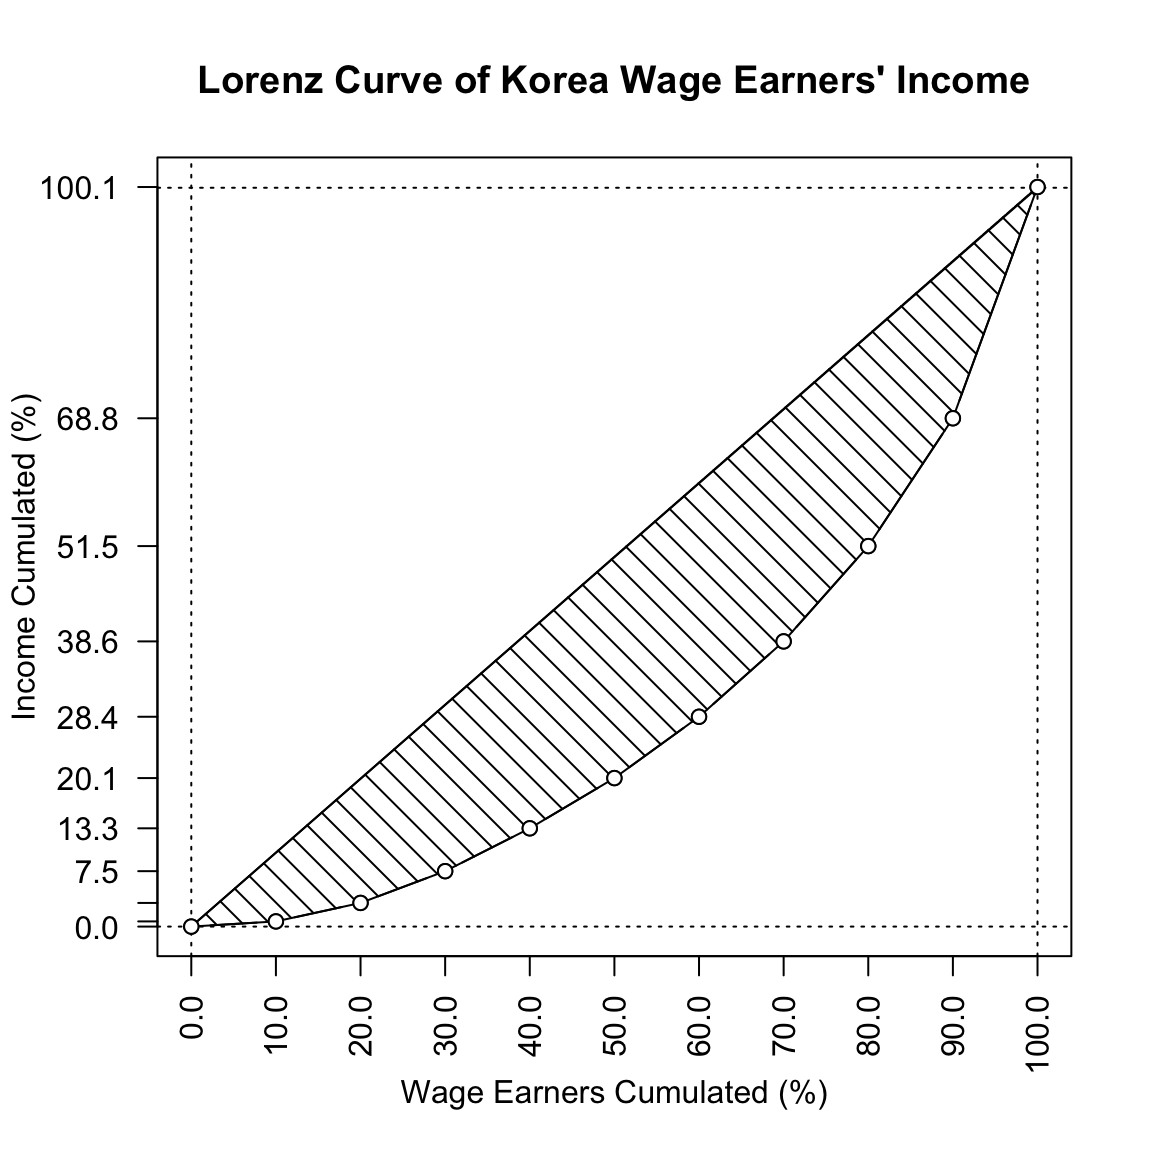
\includegraphics{Korea_Income_gini_2010_files/figure-latex/unnamed-chunk-10-1.pdf}

\hypertarget{cumulative-distribution}{%
\subsection{Cumulative distribution}\label{cumulative-distribution}}

\texttt{barplot} 보다 누적도표가 분포의 윤곽을 살피는 데 더 낫다는 점을
상기하면, 누적분포를 구하는 일부터 시작하여야 함. 자료로부터 이미 아는
사실이지만, \texttt{cumsum()}함수의 활용겸 확인차 계산해보면

\begin{verbatim}
income_kr_cum <- apply(income_kr, 
                       MARGIN = 2, 
                       FUN = cumsum)
\end{verbatim}

누적도표를 그리려면 첫 좌표는 \texttt{(0,\ 0)}이어야 함에 유의. 마침
\texttt{income\_breaks} 와 맞춰보면 \texttt{income\_kr\_cum}의 첫 행을
0으로만 추가해 주면 되는 일임.

\begin{verbatim}
income_kr_cum <- rbind(rep(0, 2), income_kr_cum)
\end{verbatim}

누적분포의 각 계급은 \texttt{10\ -\ 20}의 열리고 닫힌 구간이 아니라 한
쪽으로 열린 구간이어야 하고, 누적백분률임을 명시하려면

\begin{verbatim}
income_class_cum <- strsplit(rownames(income_kr_cum), 
                             split = " - ")
income_class_cum <- sapply(income_class_cum, 
                           FUN = function(x){x[2]})
income_class_cum <- paste("0 ~", income_class_cum)
income_class_cum[c(1, 14)] <- c("~ 0", "0 ~ 2000")
rownames(income_kr_cum) <- income_class_cum
colnames(income_kr_cum) <- c("Cumulated Wage Earners (%)", "Cumulated Income (%)")
income_kr_cum
\end{verbatim}

\begin{verbatim}
##          Cumulated Wage Earners (%) Cumulated Income (%)
## ~ 0                             0.0                  0.0
## 0 ~ 5                          19.1                  1.7
## 0 ~ 10                         31.4                  5.3
## 0 ~ 20                         54.2                 18.1
## 0 ~ 30                         68.6                 31.7
## 0 ~ 40                         78.4                 44.7
## 0 ~ 60                         90.4                 67.2
## 0 ~ 80                         95.8                 81.3
## 0 ~ 100                        98.1                 89.1
## 0 ~ 200                        99.7                 96.8
## 0 ~ 300                        99.8                 98.0
## 0 ~ 500                        99.9                 98.8
## 0 ~ 1000                       99.9                 99.4
## 0 ~ 2000                       99.9                100.0
\end{verbatim}

\begin{verbatim}
earners_kor_cum_df <- data.frame(x = income_breaks, y = income_kr_cum[, 1])
income_kr_cum_df <- data.frame(x = income_breaks, y = income_kr_cum[, 2])
\end{verbatim}

\texttt{xlim} 을 좁혀가면서 분포 윤곽 파악.

\begin{verbatim}
par(mfrow = c(2, 2))
title_2 <- "Cumulative Income Earners' Distribution"
xlab_2 <- "Income (Million Won)"
ylab_2 <- "Cumulative % of Wage Earners"
plot(earners_kor_cum_df, 
     type = "b", 
     ann = FALSE)
title(main = title_2, 
      xlab = xlab_2, 
      ylab = ylab_2)
plot(earners_kor_cum_df, 
     type = "b", 
     xlim = c(0, 500), 
     ann = FALSE)
title(main = title_2, 
      xlab = xlab_2, 
      ylab = ylab_2)
plot(earners_kor_cum_df, 
     type = "b", 
     xlim = c(0, 200), 
     ann = FALSE)
title(main = title_2, 
      xlab = xlab_2, 
      ylab = ylab_2)
plot(earners_kor_cum_df, 
     type = "b", 
     xlim = c(0, 100), 
     ann = FALSE)
title(main = title_2, 
      xlab = xlab_2, 
      ylab = ylab_2)
\end{verbatim}

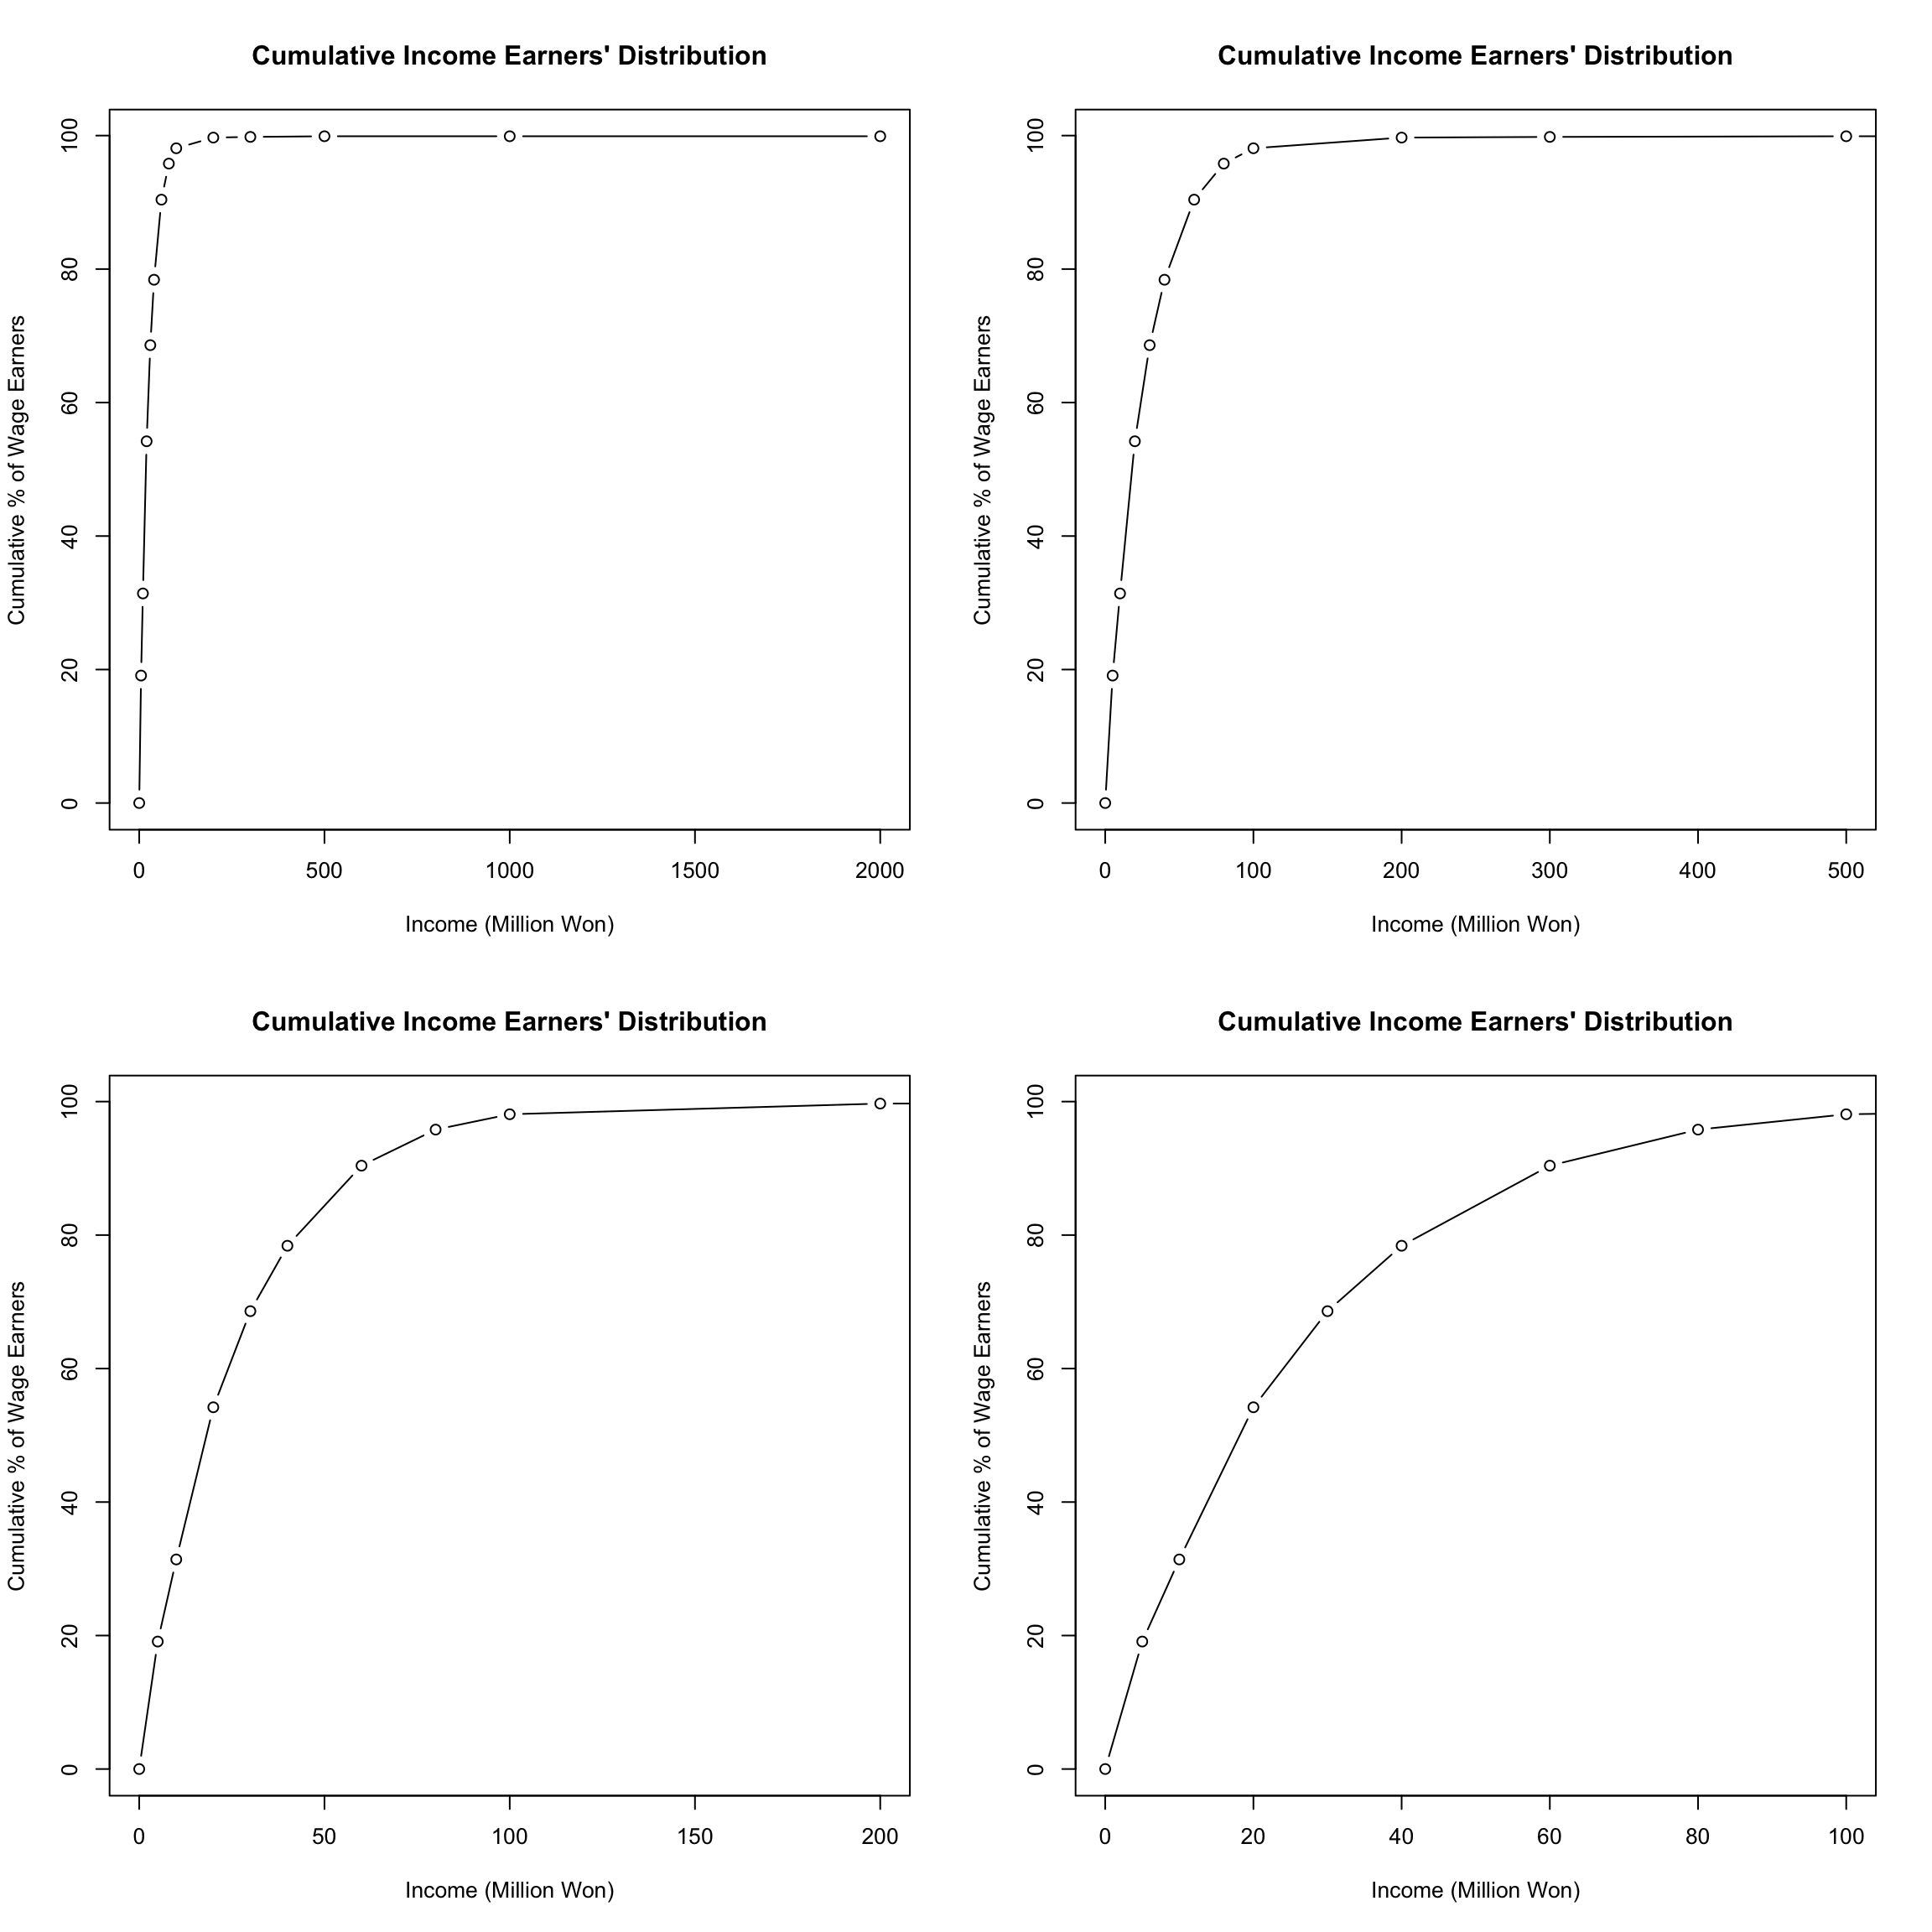
\includegraphics{Korea_Income_gini_2010_files/figure-latex/unnamed-chunk-14-1.pdf}

한가지 기억해 둘 사실은 누적분포의 윗 부분 면적이 바로 평균이라는 점.
누적분포가 히스토그램보다 나은 점 중의 하나가 분위를 찾기 쉬울 뿐 아니라
평균을 비교하는 것도 용이하다는 것임. 중위소득은 바로 \(y\)축에서 50\%에
해당하는 값을 수평으로 그은 후 누적도표와 만나는 점의 \(x\)좌표이다.
여기서 계산해 보면
\(\frac{x-10}{50 - 31.4} = \frac{54.2 - 31.4}{20 - 10}\)로부터
\(x = 18.2\)가 계산된다.

\begin{verbatim}
plot(earners_kor_cum_df, 
     type = "b", 
     xlim = c(0, 200), 
     ann = FALSE, 
     xaxt = "n", 
     yaxt = "n")
axis(side = 1, 
     at = income_breaks, 
     labels = income_breaks)
axis(side = 2, 
     at = seq(0, 100, by = 25), 
     labels = seq(0, 100, by = 25), 
     las = 1)
poly_df <- rbind(earners_kor_cum_df, c(0, 100))
polygon(poly_df, 
        density = 15, 
        angle = 135)
points(earners_kor_cum_df, 
       pch = 21, col = "black", bg = "white")
lines(x = c(0, 18.2), y = rep(50, 2), 
      col = "red", lwd = 2)
arrows(x0 = 18.2, y0 = 50, x1 = 19, y1 = 0, 
       length = 0.15, col = "red", lwd = 2)
text(x = 48, y = 25, 
     labels = "Median Income", srt = 30, col = "red")
title(main = title_2, 
      xlab = xlab_2, 
      ylab = ylab_2)
\end{verbatim}

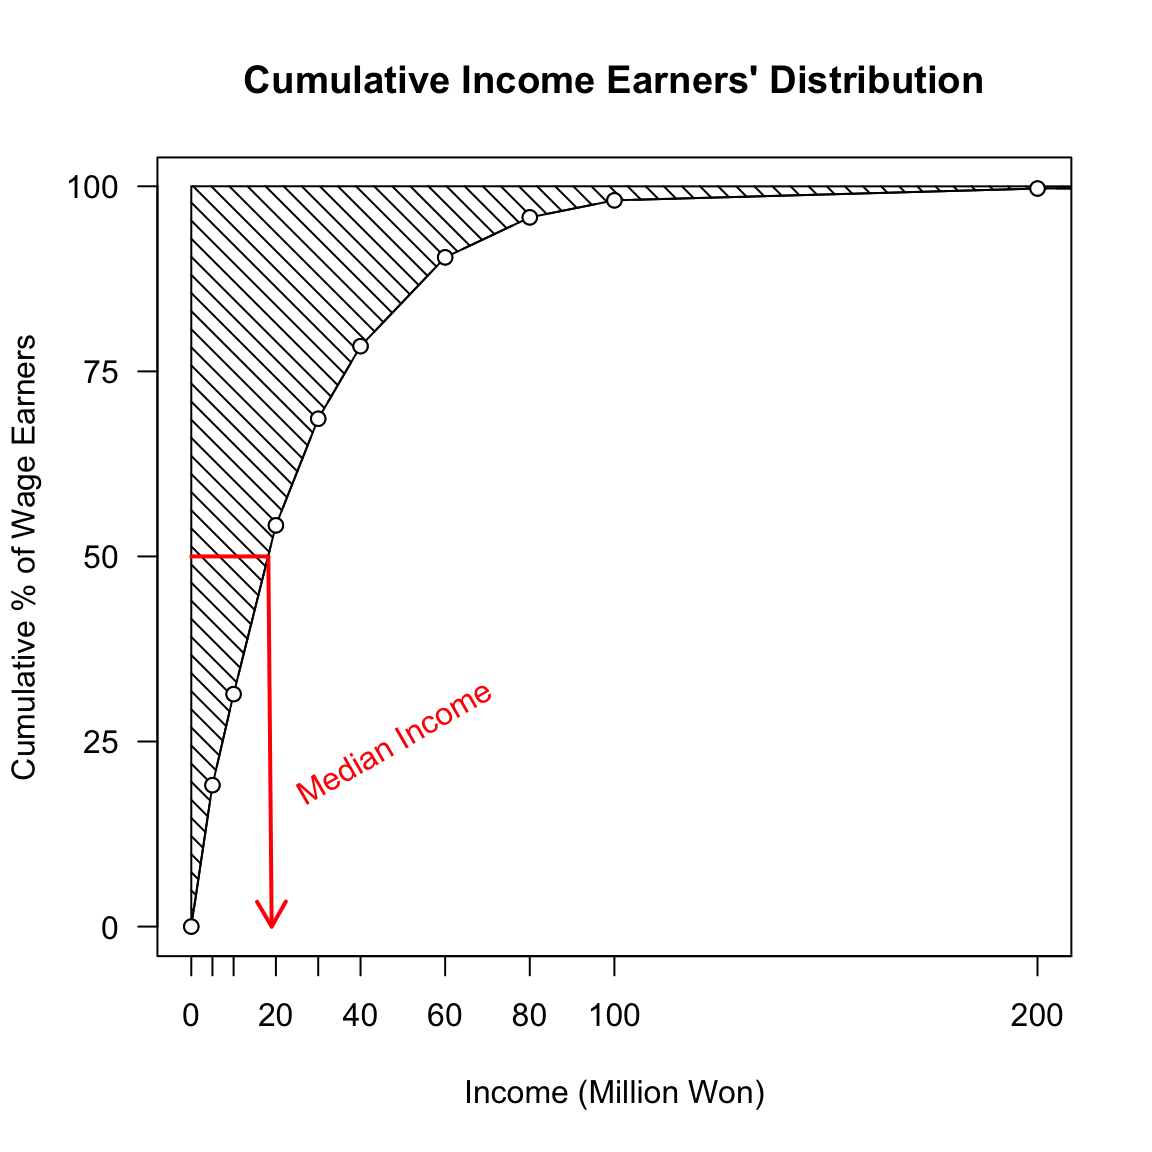
\includegraphics{Korea_Income_gini_2010_files/figure-latex/unnamed-chunk-15-1.pdf}

소득 자체의 누적분포에 대해서도 같은 방법으로 그려보면

\begin{verbatim}
par(mfrow = c(2, 2))
title_3 <- "Cumulative Income Distribution"
ylab_3 <- "Cumulative % of Income"
plot(income_kr_cum_df, 
     type = "b", 
     ann = FALSE)
title(main = title_3, 
      xlab = xlab_2, 
      ylab = ylab_3)
plot(income_kr_cum_df, 
     type = "b", 
     ann = FALSE, 
     xlim = c(0, 500))
title(main = title_3, 
      xlab = xlab_2, 
      ylab = ylab_3)
plot(income_kr_cum_df, 
     type = "b", 
     ann = FALSE, 
     xlim = c(0, 200))
title(main = title_3, 
      xlab = xlab_2, 
      ylab = ylab_3)
plot(income_kr_cum_df, 
     type = "b", 
     ann = FALSE, 
     xlim = c(0, 100))
abline(h = 89.1, 
       lty = 3, col = "red")
axis(side = 2, 
     at = 89.1, 
     label = 89.1, 
     las = 1)
title(main = title_3, 
      xlab = xlab_2, 
      ylab = ylab_3)
\end{verbatim}

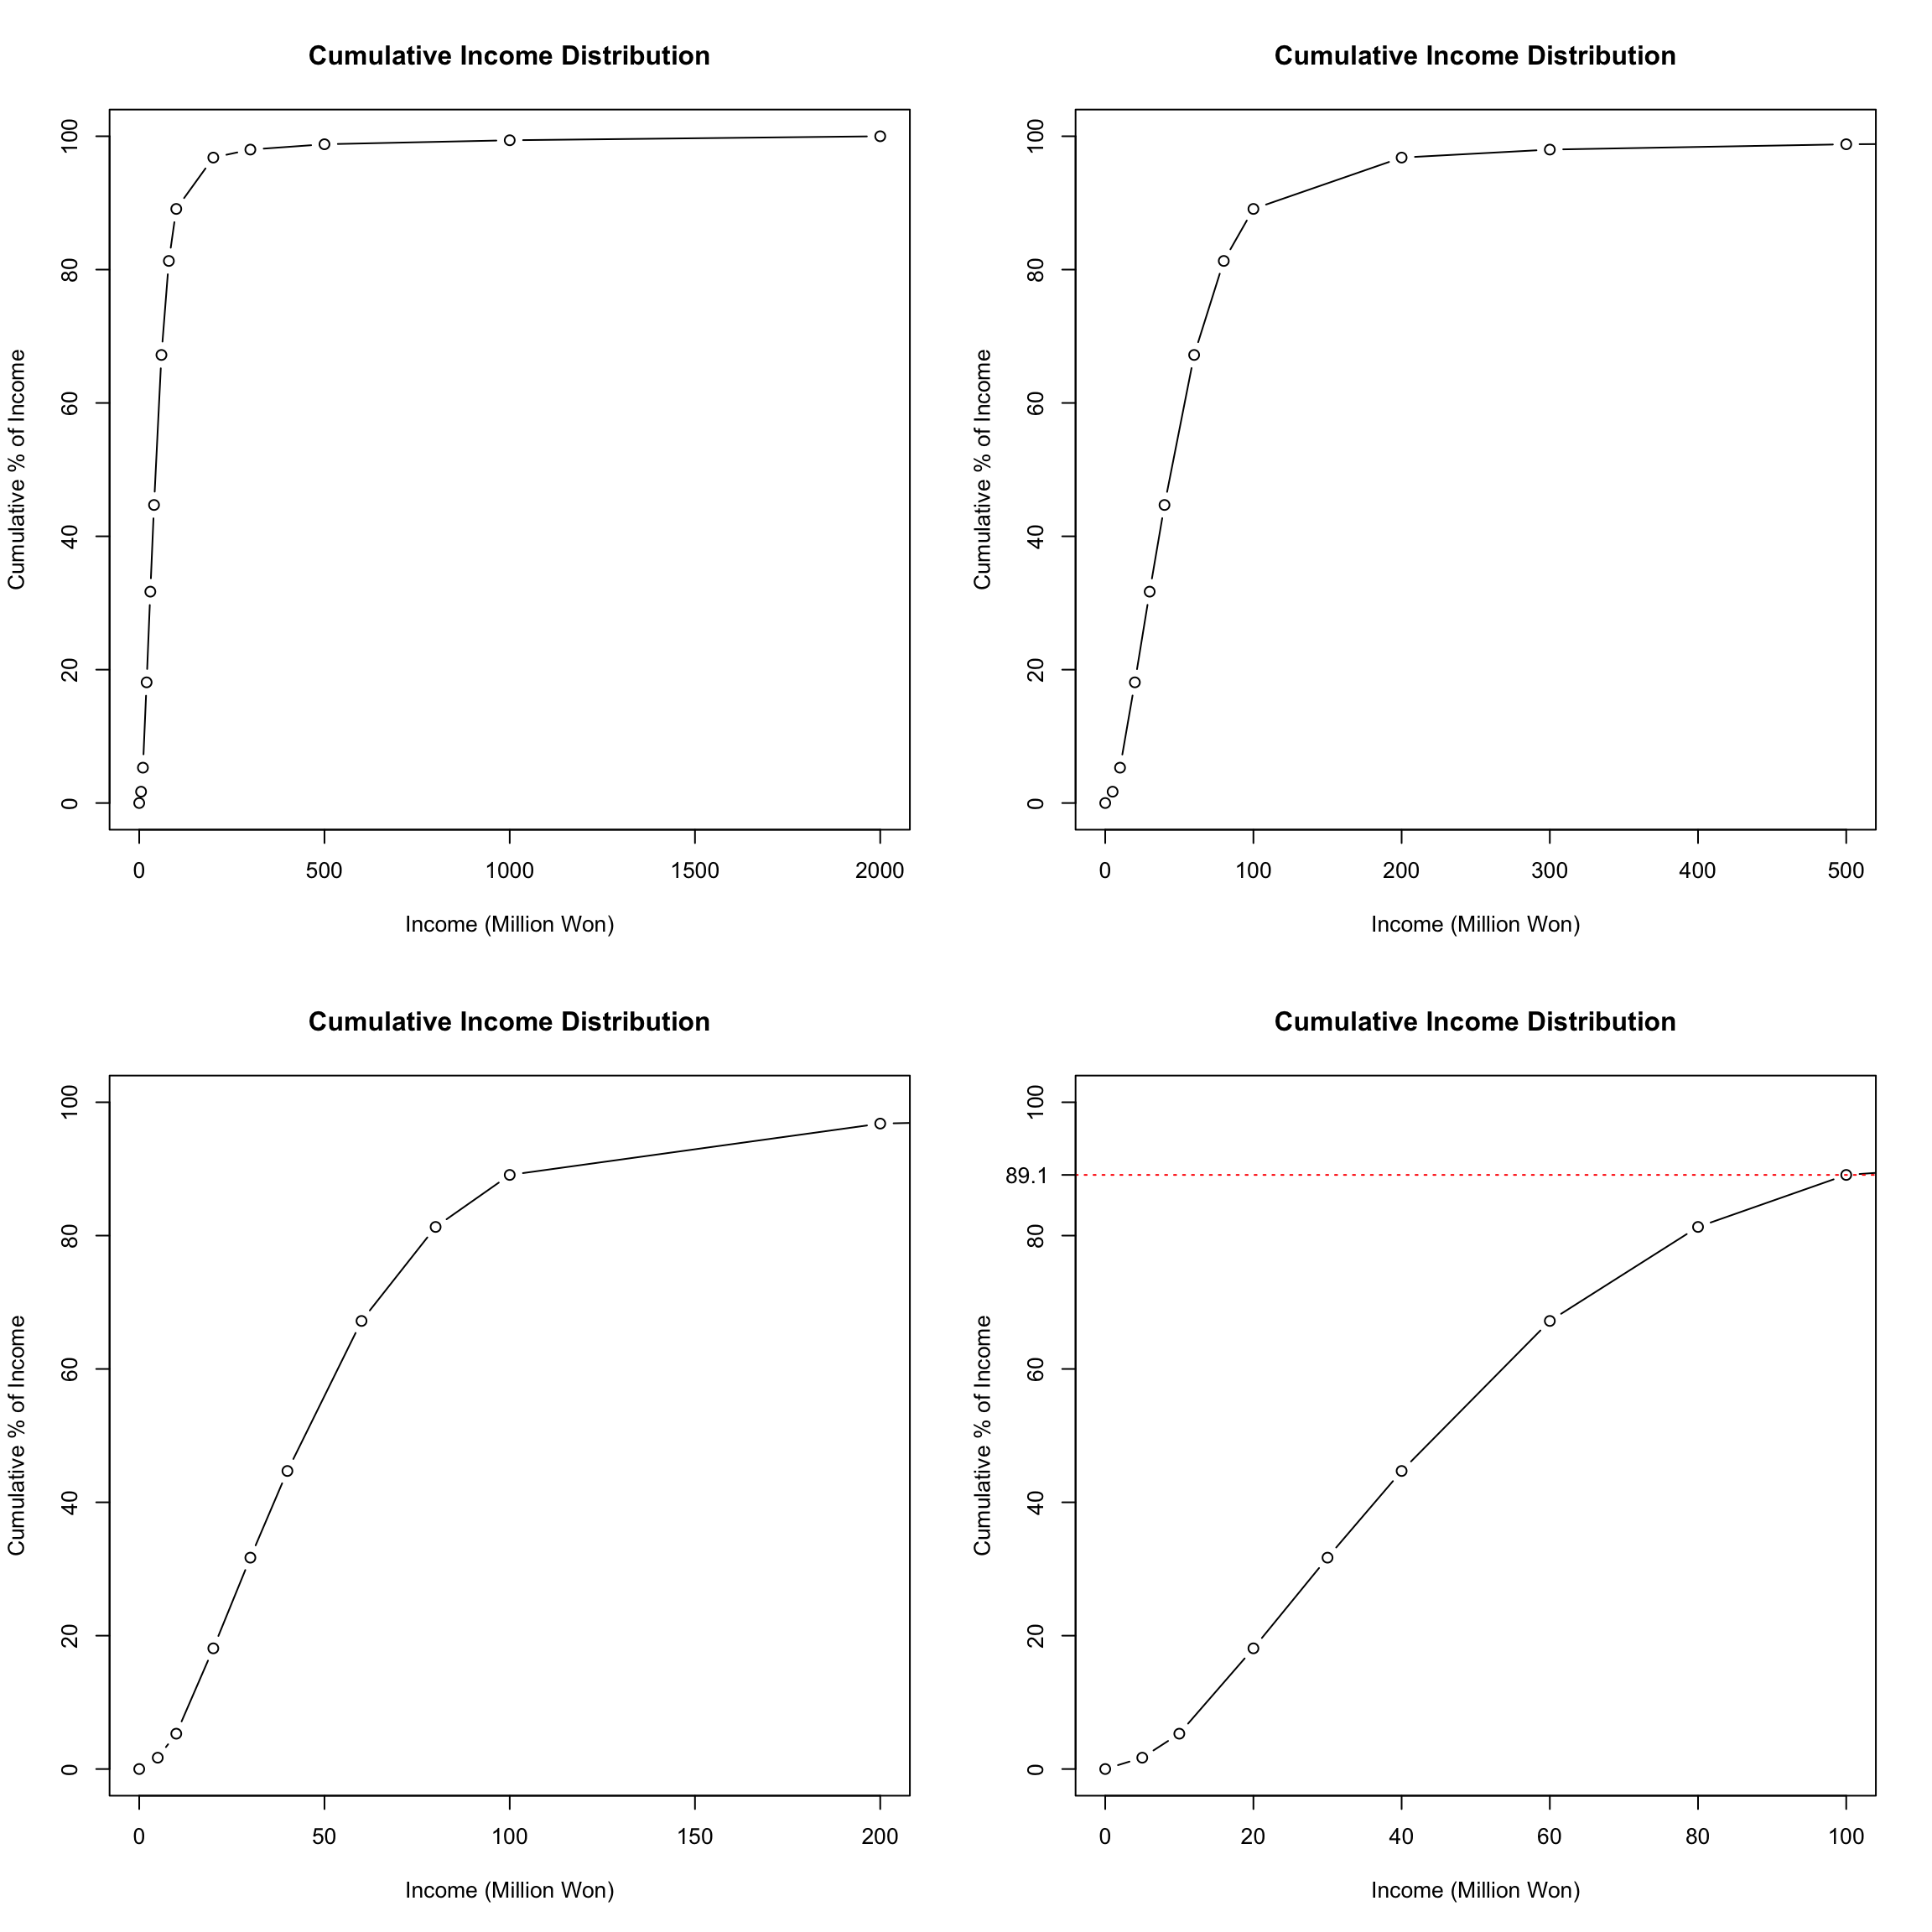
\includegraphics{Korea_Income_gini_2010_files/figure-latex/unnamed-chunk-16-1.pdf}

\hypertarget{lorenz-curve}{%
\subsection{Lorenz Curve}\label{lorenz-curve}}

이제 두 누적분포를 한 장의 도표로 살피는 방법을 생각해보자. \(x\) 축을
사람, \(y\) 축을 소득으로 하여 두 점을 이어주면 어떤 결과가 나오는 지
살펴 보자.

\begin{verbatim}
earners <- income_kr_cum[, 1] 
income <- income_kr_cum[, 2]
earners_income_df <- data.frame(Earners = earners, Income = income)
plot(earners_income_df, 
     type = "b", 
     ann = FALSE, 
     xaxt = "n", 
     yaxt = "n")
# abline(a = 0, b = 1, xlim = c(0, 100), ylim = c(0, 100))
lines(x = c(0, 100), y = c(0, 100), type = "l")
axis(side = 1, 
     at = earners, 
     labels = earners)
axis(side = 2, 
     at = income, 
     labels = income)
abline(h = c(0, 100), lty = 3)
abline(v = c(0, 100), lty = 3)
title_4 <- "Lorenz Curve of Korea Wage Earners' Income"
xlab_4 <- "Wage Earners Cumulated (%)"
ylab_4 <- "Income Cumulated (%)"
title(main = title_4, 
      xlab = xlab_4, 
      ylab = ylab_4)
\end{verbatim}

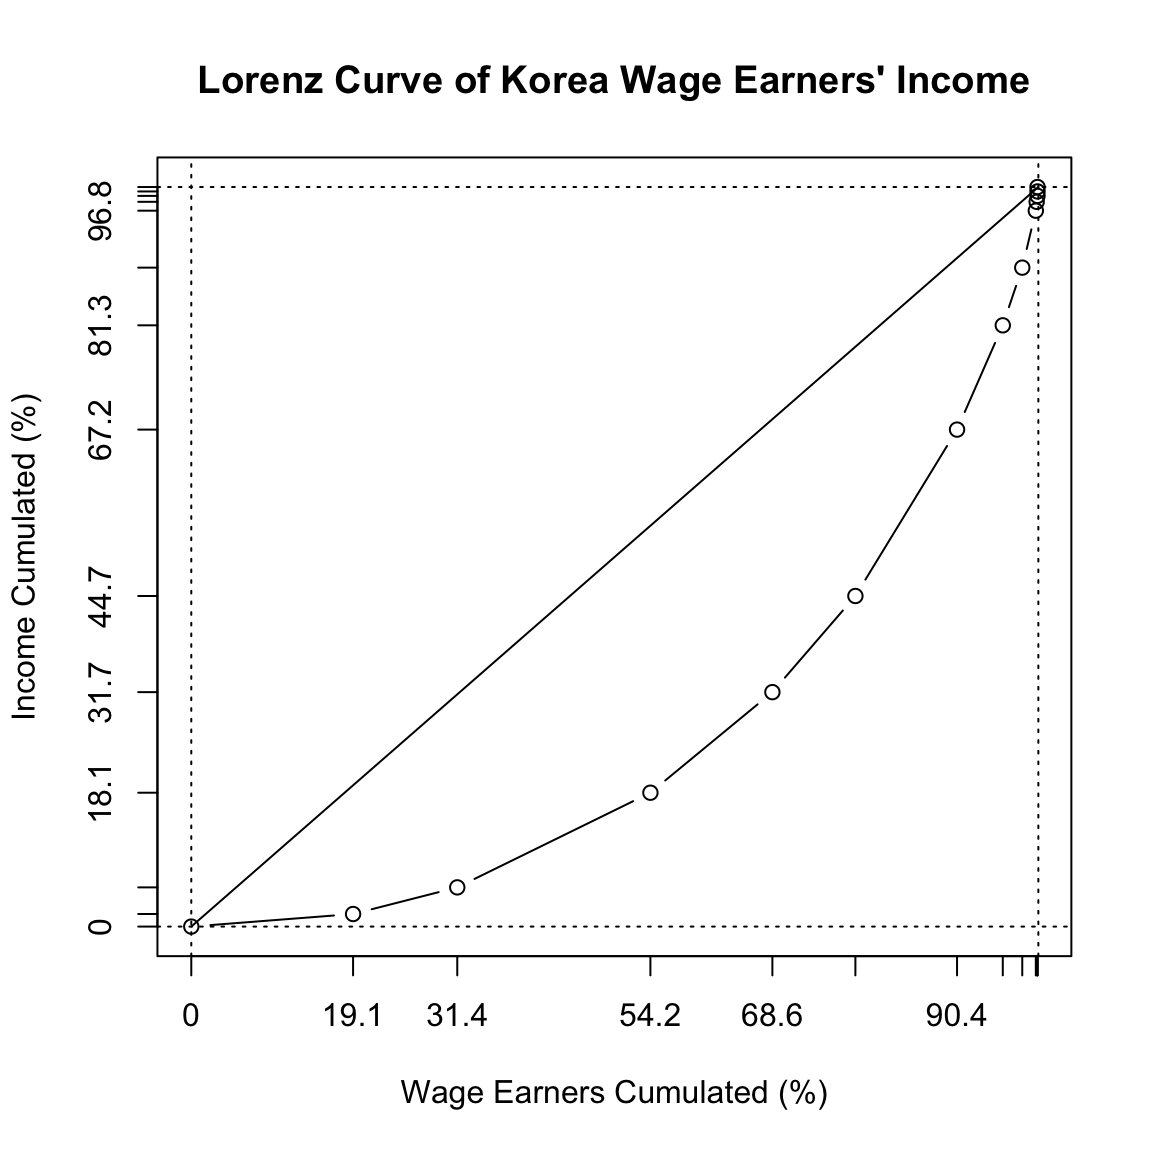
\includegraphics{Korea_Income_gini_2010_files/figure-latex/unnamed-chunk-17-1.pdf}

초승달 부분에 빗금을 치고, 각 축의 눈금을 가능한 많이 표시하려면
\texttt{polygon()}과 \texttt{axis(...,\ las\ =\ )}을 이용하게 되는 데 이
때 다각형을 구성하는데 필요한 좌표들은 이미
\texttt{earners\_income\_df}에 모두 나와 있음.

\begin{verbatim}
plot(earners_income_df, 
     type = "b", 
     ann = FALSE, 
     xaxt = "n", 
     yaxt = "n")
# abline(a = 0, b = 1, xlim = c(0, 100), ylim = c(0, 100))
lines(x = c(0, 100), y = c(0, 100), type = "l")
axis(side = 1, 
     at = earners, 
     labels = format(earners, nsmall = 1))
axis(side = 2, 
     at = income[c(1:10, 14)], 
     labels = format(income[c(1:10, 14)], nsmall = 1), 
     las = 1)
abline(h = c(0, 100), lty = 3)
abline(v = c(0, 100), lty = 3)
title(main = title_4, 
      xlab = xlab_4, 
      ylab = ylab_4)
polygon(earners_income_df, 
        density = 10, 
        angle = 135)
points(earners_income_df, 
       pch = 21, col = "black", bg = "white")
\end{verbatim}

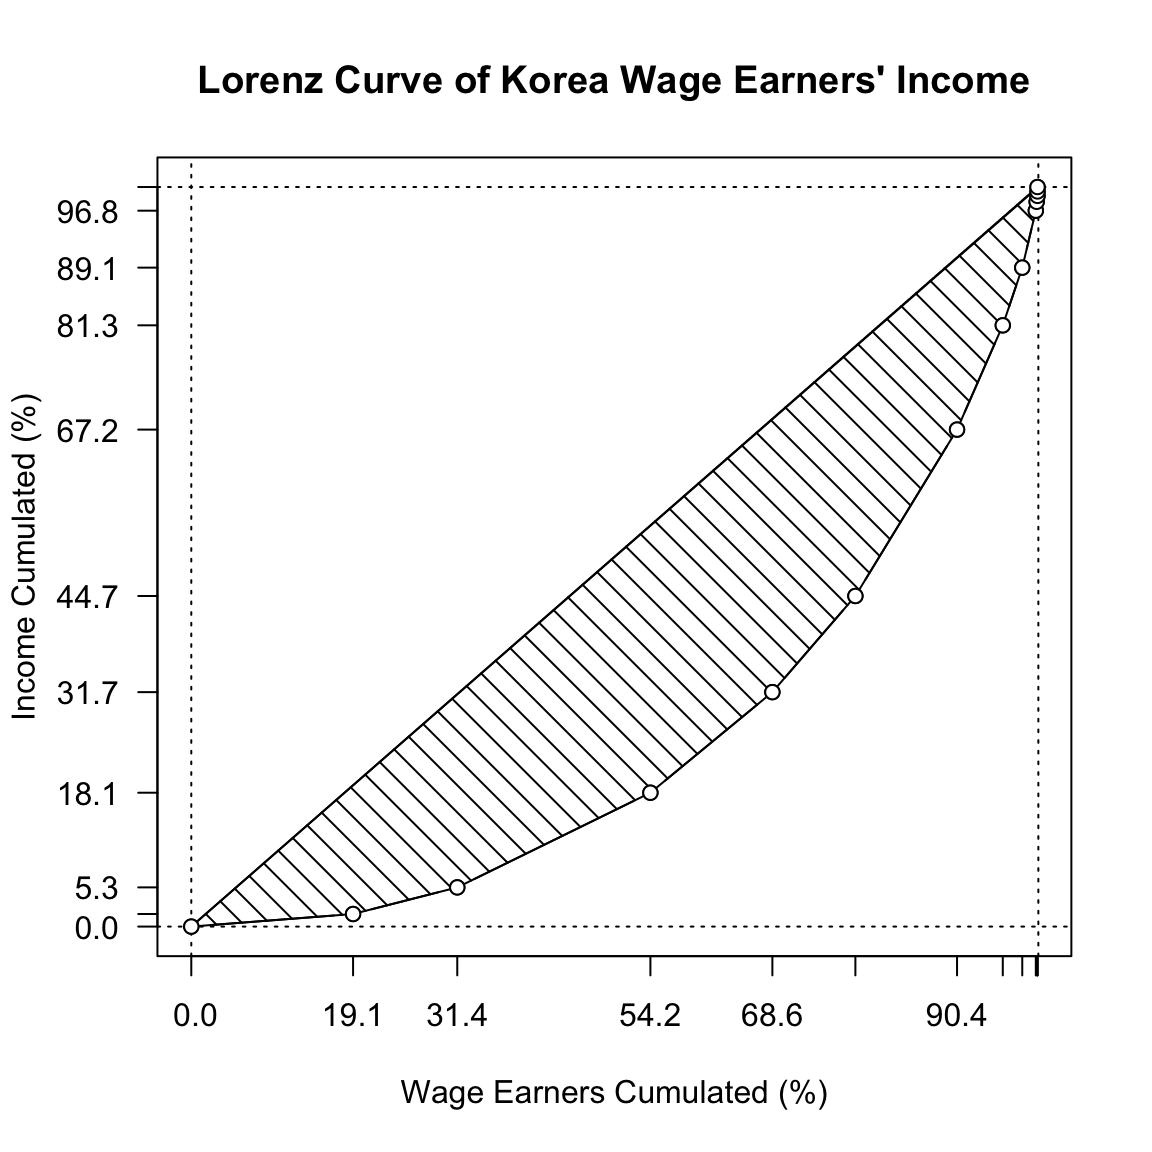
\includegraphics{Korea_Income_gini_2010_files/figure-latex/unnamed-chunk-18-1.pdf}

이 곡선의 이름은 무엇인가요?
\href{https://en.wikipedia.org/wiki/Lorenz_curve}{Lorenz Curve} 참조.

\hypertarget{gini-coefficient}{%
\subsubsection{Gini coefficient}\label{gini-coefficient}}

지니계수는 완전평등선과 로렌츠 곡선 사이의 면적을 완전불평등 상황에서의
면적, 즉 1/2로 나눠 준 값이다. 이 값이 클수록 불평등이 심한 것으로
간주할 수 있다. 이 초승달 모양 면적은 삼각형 면적에서 로렌츠 곡선 아래
면적을 뺀 것과 같아지므로 이전에 작성한 \texttt{arae\_R}함수를 이용할 수
있다.

\begin{verbatim}
source("area.R")
gini <- 2 * (1/2 - area_R(x = earners, y = income)/10000)
\end{verbatim}

계산된 지니계수를 그림 안에 텍스트로 넣어주려면 \texttt{paste()}를
이용하여 입력토록한다.

\begin{verbatim}
plot(earners_income_df, 
     type = "b", 
     ann = FALSE, 
     xaxt = "n", 
     yaxt = "n")
lines(x = c(0, 100), y = c(0, 100), type = "l")
axis(side = 1, 
     at = earners, 
     labels = format(earners, nsmall = 1))
axis(side = 2, 
     at = income[c(1:10, 14)], 
     labels = format(income[c(1:10, 14)], nsmall = 1), 
     las = 1)
abline(h = c(0, 100), lty = 3)
abline(v = c(0, 100), lty = 3)
title(main = title_4, 
      xlab = xlab_4, 
      ylab = ylab_4)
polygon(earners_income_df, 
        density = 10, 
        angle = 135)
points(earners_income_df, 
       pch = 21, col = "black", bg = "white")
text(x = 30, y = 60, 
     labels = paste("Gini = ", round(gini, digits = 3)), cex = 1.5)
\end{verbatim}

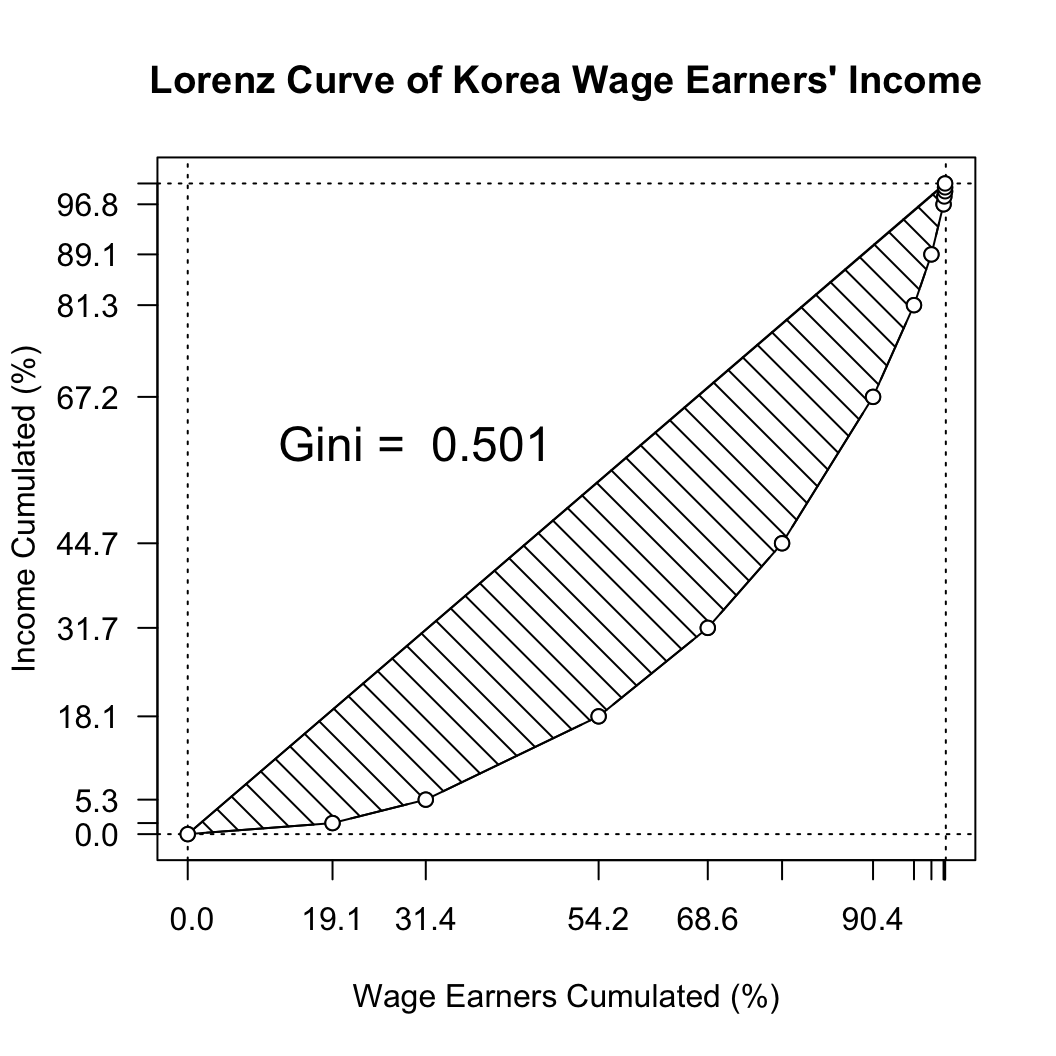
\includegraphics{Korea_Income_gini_2010_files/figure-latex/unnamed-chunk-19-1.pdf}

\hypertarget{ggplot}{%
\subsection{ggplot}\label{ggplot}}

단계별로 결과물을 저장하면서 작업할 수 있도록 구성하였으니
\texttt{fig.keep\ =\ \textquotesingle{}none\textquotesingle{}} 를
\texttt{fig.keep\ =\ \textquotesingle{}all\textquotesingle{}}로 바꿔서
실행시켜보면 각 단계에서 어떤 점이 추가되는 지 살필 수 있다.

\hypertarget{cumulative-distribution-1}{%
\subsubsection{Cumulative
Distribution}\label{cumulative-distribution-1}}

\begin{verbatim}
library(ggplot2)
(c1 <- ggplot() +
  geom_line(data = earners_kor_cum_df, 
            mapping = aes(x = x, y = y), na.rm = TRUE))
(c2 <- c1 +
  scale_x_continuous(breaks = earners_kor_cum_df$x,
                     labels = earners_kor_cum_df$x,
                     limits = c(0, 200)))
(c3 <- c2 +
  geom_hline(yintercept = c(0, 100), linetype = "dotted")) 
(c4 <- c3 +
  geom_vline(xintercept = c(0, 200), linetype = "dotted")) 
(c5 <- c4 + 
  geom_polygon(data = poly_df[-(11:14), ], 
               mapping = aes(x = x, y = y), 
               alpha = 0.5, fill = "grey")) 
(c6 <- c5 +
  geom_point(data = earners_kor_cum_df, 
             mapping = aes(x = x, y = y), 
             shape = 21, fill = "white", size = 3,
             na.rm = TRUE)) 
(c7 <- c6 +
  ggtitle(title_2) + xlab(xlab_2) + ylab(ylab_2)) 
(c8 <- c7 +
  scale_y_continuous(breaks = seq(0, 100, by = 25), labels = seq(0, 100, by = 25)))
(c9 <- c8 +
    annotate("segment", x = 0, xend = 18.2, y = 50, yend = 50, colour = "red", size = 1))
(c10 <- c9 +
    geom_segment(data = data.frame(x1 = 18.2, x2 = 18.2, y1 = 50, y2 = 0),
                 aes(x = x1, y = y1, xend = x2, yend = y2), 
                 arrow = arrow(),
                 colour = "red",
                 size = 1))
(c11 <- c10 +
  annotate("text", x = 55, y = 25, 
           label = "Median Income", size = 5, color = "red", srt = 15)) 
(c12 <- c11 +
  theme_bw() +
    theme(plot.title = element_text(hjust = 0.5, size = 15)))
\end{verbatim}

\begin{verbatim}
c12
\end{verbatim}

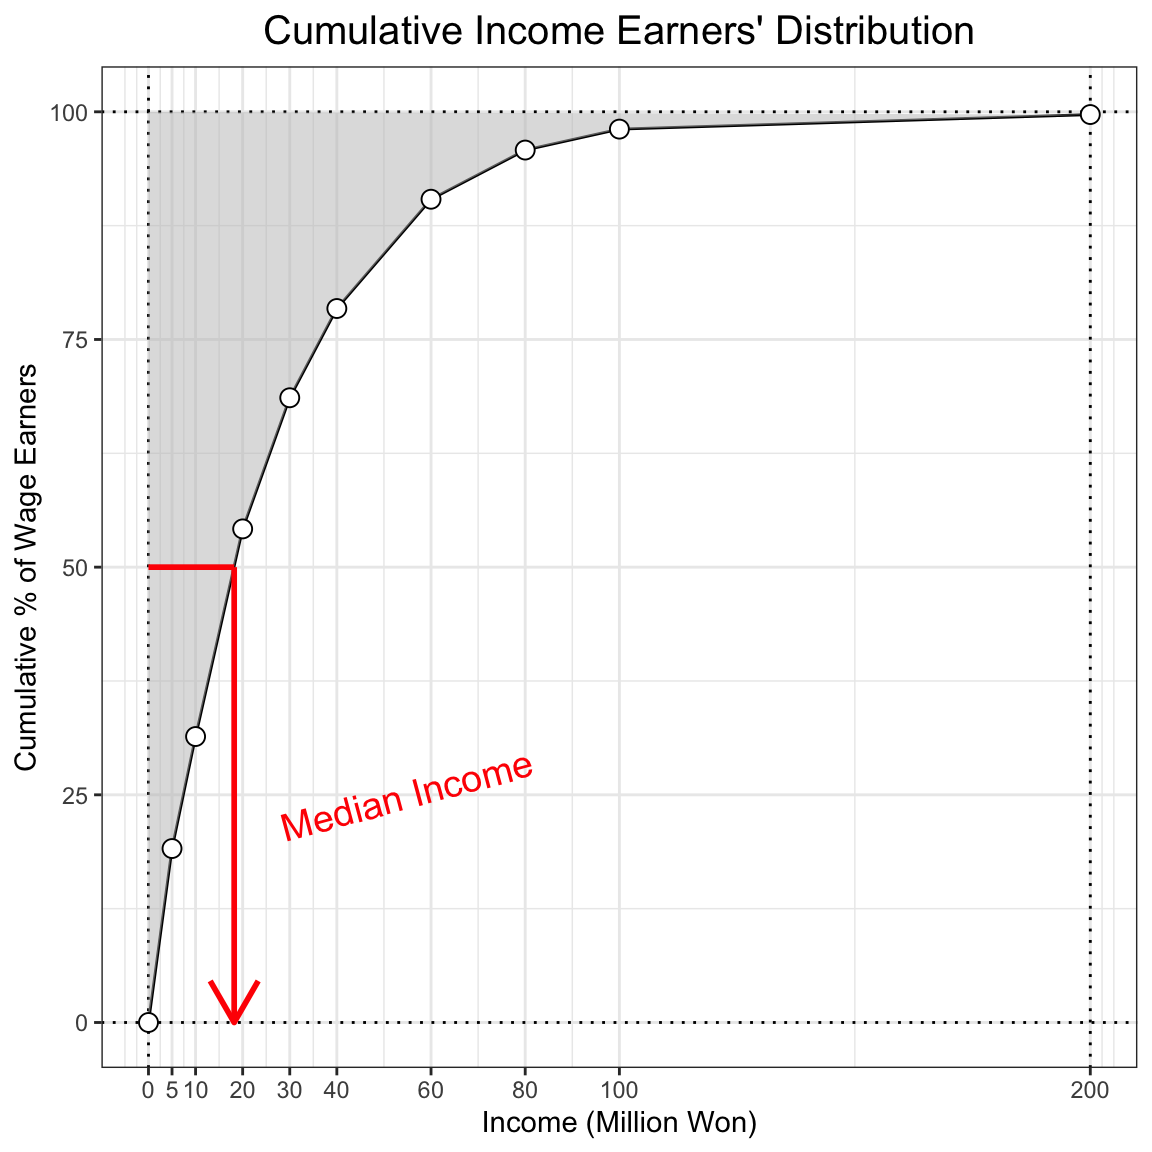
\includegraphics{Korea_Income_gini_2010_files/figure-latex/unnamed-chunk-21-1.pdf}

\begin{verbatim}
ggsave("../pics/cumulative_plot_wage_kr.png", width = 9, height = 9)
\end{verbatim}

\hypertarget{lorenz-curve-1}{%
\subsubsection{Lorenz Curve}\label{lorenz-curve-1}}

\begin{verbatim}
(g1 <- ggplot() +
  geom_line(data = earners_income_df, 
            mapping = aes(x = earners, y = income))) 
(g2 <- g1 +
  geom_line(data = data.frame(x = c(0, 100), y = c(0, 100)), 
            mapping = aes(x = x, y = y))) 
(g3 <- g2 +
  geom_hline(yintercept = c(0, 100), linetype = "dotted")) 
(g4 <- g3 +
  geom_vline(xintercept = c(0, 100), linetype = "dotted")) 
(g5 <- g4 + 
  geom_polygon(data = earners_income_df, 
               mapping = aes(x = earners, y = income), 
               alpha = 0.5, fill = "grey")) 
(g6 <- g5 +
  geom_point(data = earners_income_df, 
             mapping = aes(x = earners, y = income), 
             shape = 21, fill = "white", size = 3)) 
(g7 <- g6 +
  labs(title = title_4, x = xlab_4, y = ylab_4))
(g8 <- g7 +
  scale_x_continuous(breaks = earners[c(1:8, 14)], 
                     labels = format(earners[c(1:8, 14)], nsmall = 1))) 
(g9 <- g8 +
  scale_y_continuous(breaks = income[c(1:8, 14)], 
                     labels = format(income[c(1:8, 14)], nsmall = 1)))
#  scale_y_continuous(breaks = seq(0, 100, by = 25))) 
(g10 <- g9 +
  annotate("text", x = 30, y = 60, 
           label = paste("Gini = ", format(gini, digits = 3, nsmall = 2)), 
           size = 9, color = "red", srt = 15)) 
(g11 <- g10 +
  annotate("text", x = 80, y = 20, 
           label = "15 Million", 
           size = 9, color = "blue"))
(g12 <- g11 +
  theme_bw() +
    theme(plot.title = element_text(hjust = 0.5, size = 15)))
\end{verbatim}

\begin{verbatim}
g12
\end{verbatim}

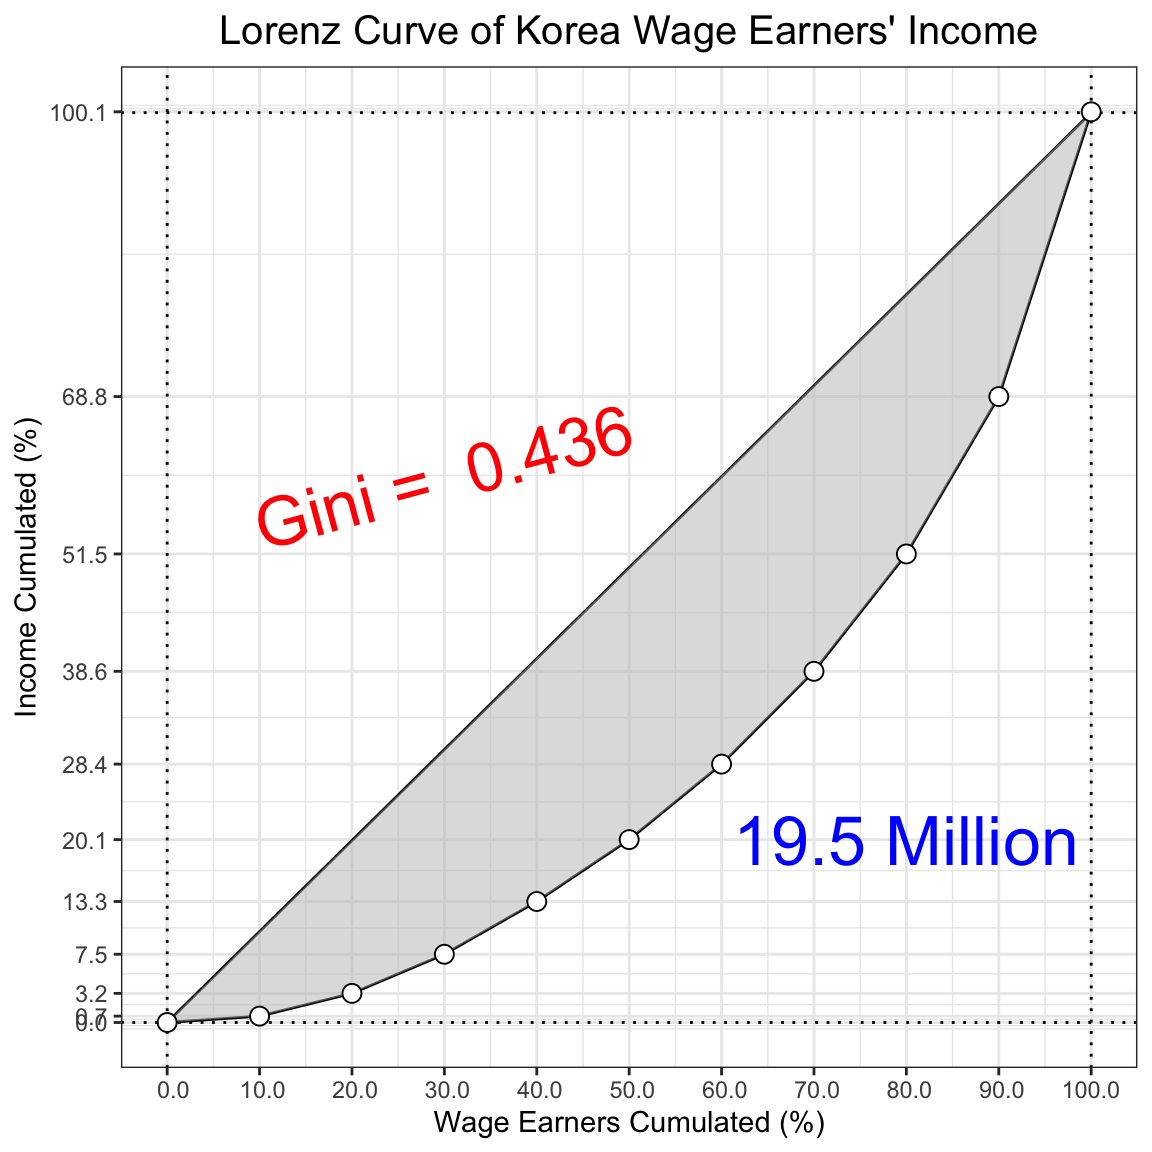
\includegraphics{Korea_Income_gini_2010_files/figure-latex/final output-1.pdf}

\begin{verbatim}
ggsave("../pics/lorenz_curve_wage_kr.png", width = 9, height = 9)
\end{verbatim}

\end{document}
